\documentclass[../notes.tex]{subfiles}
\graphicspath{{\subfix{../images/}}, {\subfix{../}}}

\begin{document}
\raggedbottom
	
\chapter{Introduction}

The United Nations declared 2025 the `International Year of Quantum Science and Technology' \cite{unitednationsInternationalYearQuantum2024}.
This is an effort is to raise awareness of the importance of quantum science and its applications, which focuses in 3 key areas: quantum computing, quantum communications and quantum sensors.
One effect underlying many of these applications is the phenomenon of superconductivity.
For example, superconducting qubits are a promising platform for scalable quantum computing \cite{huangSuperconductingQuantumComputing2020, aruteQuantumSupremacyUsing2019} and the Josephson effect \cite{josephsonPossibleNewEffects1962} can be used to build extremely sensitive measurement devices for magnetic fields \cite{faleyHighTcSQUIDBiomagnetometers2017} or voltages \cite{klushinPresentFutureHightemperature2020}.

Superconductivity was discovered in 1911, when Heike Onnes measured that the electrical resistance of Mercury suddenly vanished completely when cooling it below \qty{4}{\kelvin} \cite{onnesFurtherExperimentsLiquid1991}.
In the following decades, more effects in superconducting materials were discovered such as the Meissner effect, the perfect expulsion of external magnetic fields \cite{meissnerNeuerEffektBei1933}.
The theoretical description 

\todo{Description: macroscopic quantum mechanics}

\todo{BCS theory}

%As such, superconductivity is one of the important examples of quantum mechanical effects manifesting on a macroscopical scale.


\subsection*{Unconventional Superconductivity}

In 1986 and 1987, superconductivity with very high \(T_C\) of \qty{30}{\kelvin} (the highest \(T_C\) until then was \qty{23.7}{\kelvin} in \ce{Nb3Ge}) was discovered in cuprates \cite{bednorzPossibleHighTc1986,uchidaHighTcSuperconductivity1987}.
Cuprate superconductors are made up of layers of cooper oxide and charge reservoirs in between.
The specific charge reservoir layers determine the properties of the superconducting and varying them lead to the discovery of a rich zoo of materials with high \(T_C\) \cite{rybickiPerspectivePhaseDiagram2016}.
Cuprates are the prime example of the class of superconductors that cannot be explained by BCS theory.
They are called unconventional.
Mechanisms of pairing are something else that the electron-phonon interaction in BCS-theory, i.e. purely electronic mechanisms.
In Cuprates, parent state is a Mott insular (insulator emerging from strong electronic correlations).
This means it cannot be explained by BCS theory, because there the parent state is a Fermi liquid.
\todo{Some more words on characterization: unconventional, high TC, strongly correlated/coupling}

HTSC not only have higher \(T_C\), so that lower-cost cooling methods can be employed, they also support stronger currents and can withstand higher magnetic fields until SC breaks down.
These three parameters span the critical surface (see \cref{fig:Critical Surface of a SC}), should be largest for technical applications.
\begin{SCfigure}[50]
	\centering
	\import{images/}{Critical Surface.pdf_tex}
	\caption{\textbf{Critical surface of a superconductor.} For practical applications, this surface is desired to be as large as possible, making it possible to carry high currents and generate strong magnetic fields while not needing to cool the superconductor to very low temperatures. This generally is the case for high-temperature superconductors in comparison to low-temperature superconductors. }
	\label{fig:Critical Surface of a SC}
\end{SCfigure}
So for HTSC, largest commercial application to date is in magnetic resonance imaging, a medical technique using strong magnetic fields and field gradients \cite{rinckMagneticResonanceMedicine}.
There is cable development \cite{schmidtOperationExperienceFurther2012, konstantopoulouDesignOptimizationEvaluation2019} utilizing the high critical currents.

Critical currents and magnetic fields closely linked to two length scales in SCs: the coherence length \(\xi_0\) and the London penetration depth \(\lambda_{L,0}\).
Coherence length is linked to size of Cooper pairs, London penetration depth describes how far magnetic fields penetrate into a SC.
These length scales are a further characterization of SCs.
For example, SC can be split up into type I and type II.
The difference is in the response to magnetic fields.
In type I SC, sc order is destroyed for fields higher than a critical magnetic field \(H_{C}\).
Type II superconductors have two critical fields \(H_{C_1, C_2}\), \(H_{C_1} > H_{C_2}\).
For fields higher than \(H_{C_1}\), the superconducting state is completely destroyed.
For fields higher than \(H_{C_2}\) but lower than \(H_{C_1}\), the superconducting order is not destroyed, but magnetic field lines penetrate the material.
\todo{Experimental measurement of length scales}
To characterize SC materials, especially SCs with strong correlations it is very desirable to calculate the length scales in ab-initio frameworks.

\subsection*{BCS-BEC Crossover}

\begin{SCfigure}[50]
	\centering
	\includegraphics[width=0.5\textwidth]{images/BCS-BEC crossover.png}
	\caption{\textbf{BCS-BEC crossover.} Reprinted figure with permission from \cite{chenWhenSuperconductivityCrosses2024}. Copyright 2024 by the
		American Physical Society.}
	\label{fig:BCS-BEC-crossover}
\end{SCfigure}
Topic in the context of high \(T_C\) SCs.
Framework independent of pairing mechanism.
Two regimes can be connected by \todo{Regimes}

\Cref{fig:BCS-BEC-crossover} shows the \todo{describe figure}

The intermediate region is characterized by the fact that the \todo{difference between condensing and SC}

\todo{BEC regime: TC is given by DS}

\todo{Optimization of TC, need access to SC length scales}

\cite{chenWhenSuperconductivityCrosses2024}

\subsection*{Graphene Structures as a Platform for Correlated Physics}

%The last family of superconductors which we want to discuss comprises twodimensional (2D) materials. Since the successful exfoliation of graphene in 2004 [157],  the field of (quasi) 2D materials is thriving [158–160]. These materials characterize by  their unique properties arising from quantum confinement and their high tunability  via mechanisms such as environmental dielectric screening, electrostatic doping,  heterostructuring capabilities, or external field tuning

\todo{Introduction to Graphene historically}

Following the 2018 discovery of superconductivity in twisted bilayer Graphene \cite{caoUnconventionalSuperconductivityMagicangle2018}, graphene-based systems gained a renewed interest as a platform for strongly correlated physics.
Two methods to engineer strong electron correlations emerged: twisted multilayer systems  \cite{caoUnconventionalSuperconductivityMagicangle2018, tanakaSuperfluidStiffnessMagicangle2025, tormaSuperconductivitySuperfluidityQuantum2022, andreiGrapheneBilayersTwist2020, xieTopologyBoundedSuperfluidWeight2020} and multilayer systems without twisting, such as Bernal bilayer, ABC or ABCA layered systems \cite{pantaleonSuperconductivityCorrelatedPhases2023}.
Through different means, electrons in these systems become localized so that interaction effects get more strongly pronounced.
Connecting both kind of systems is the strong quantum geometry coming from the Graphene Dirac cones \cite{wehlingDiracMaterials2014}, which plays a role in stabilizing superconducting \cite{liangBandGeometryBerry2017, tanakaSuperfluidStiffnessMagicangle2025} and magnetic order \cite{abouelkomsanQuantumMetricInduced2023, liuOrbitalMagneticStates2021}.


One interesting development in is in twisted multilayer systems, first realized as twisted bilayer Graphene \cite{caoUnconventionalSuperconductivityMagicangle2018}.
In comparison to the complex crystal structure of e.g. the Cuprates, twisted multilayer systems have a very simple structure and can be tuned very easily: the angle of twist between the layers can be easily accessed experimentally.
The defining feature of these systems are flat electronic bands due to folding of the Brilluoin zone.
Superconductivity in these systems is enhanced due to the fact that in the flat bands, interactions between the electrons are very strongly enhanced.
Thus these systems are a very interesting playground to study strongly correlation effects in general and superconductivity in particular.

\begin{figure}
	\begin{subfigure}[b]{0.5\textwidth}
		\centering
		\caption{\hfill\null}\label{sfig:3D printed twisted Graphene}
		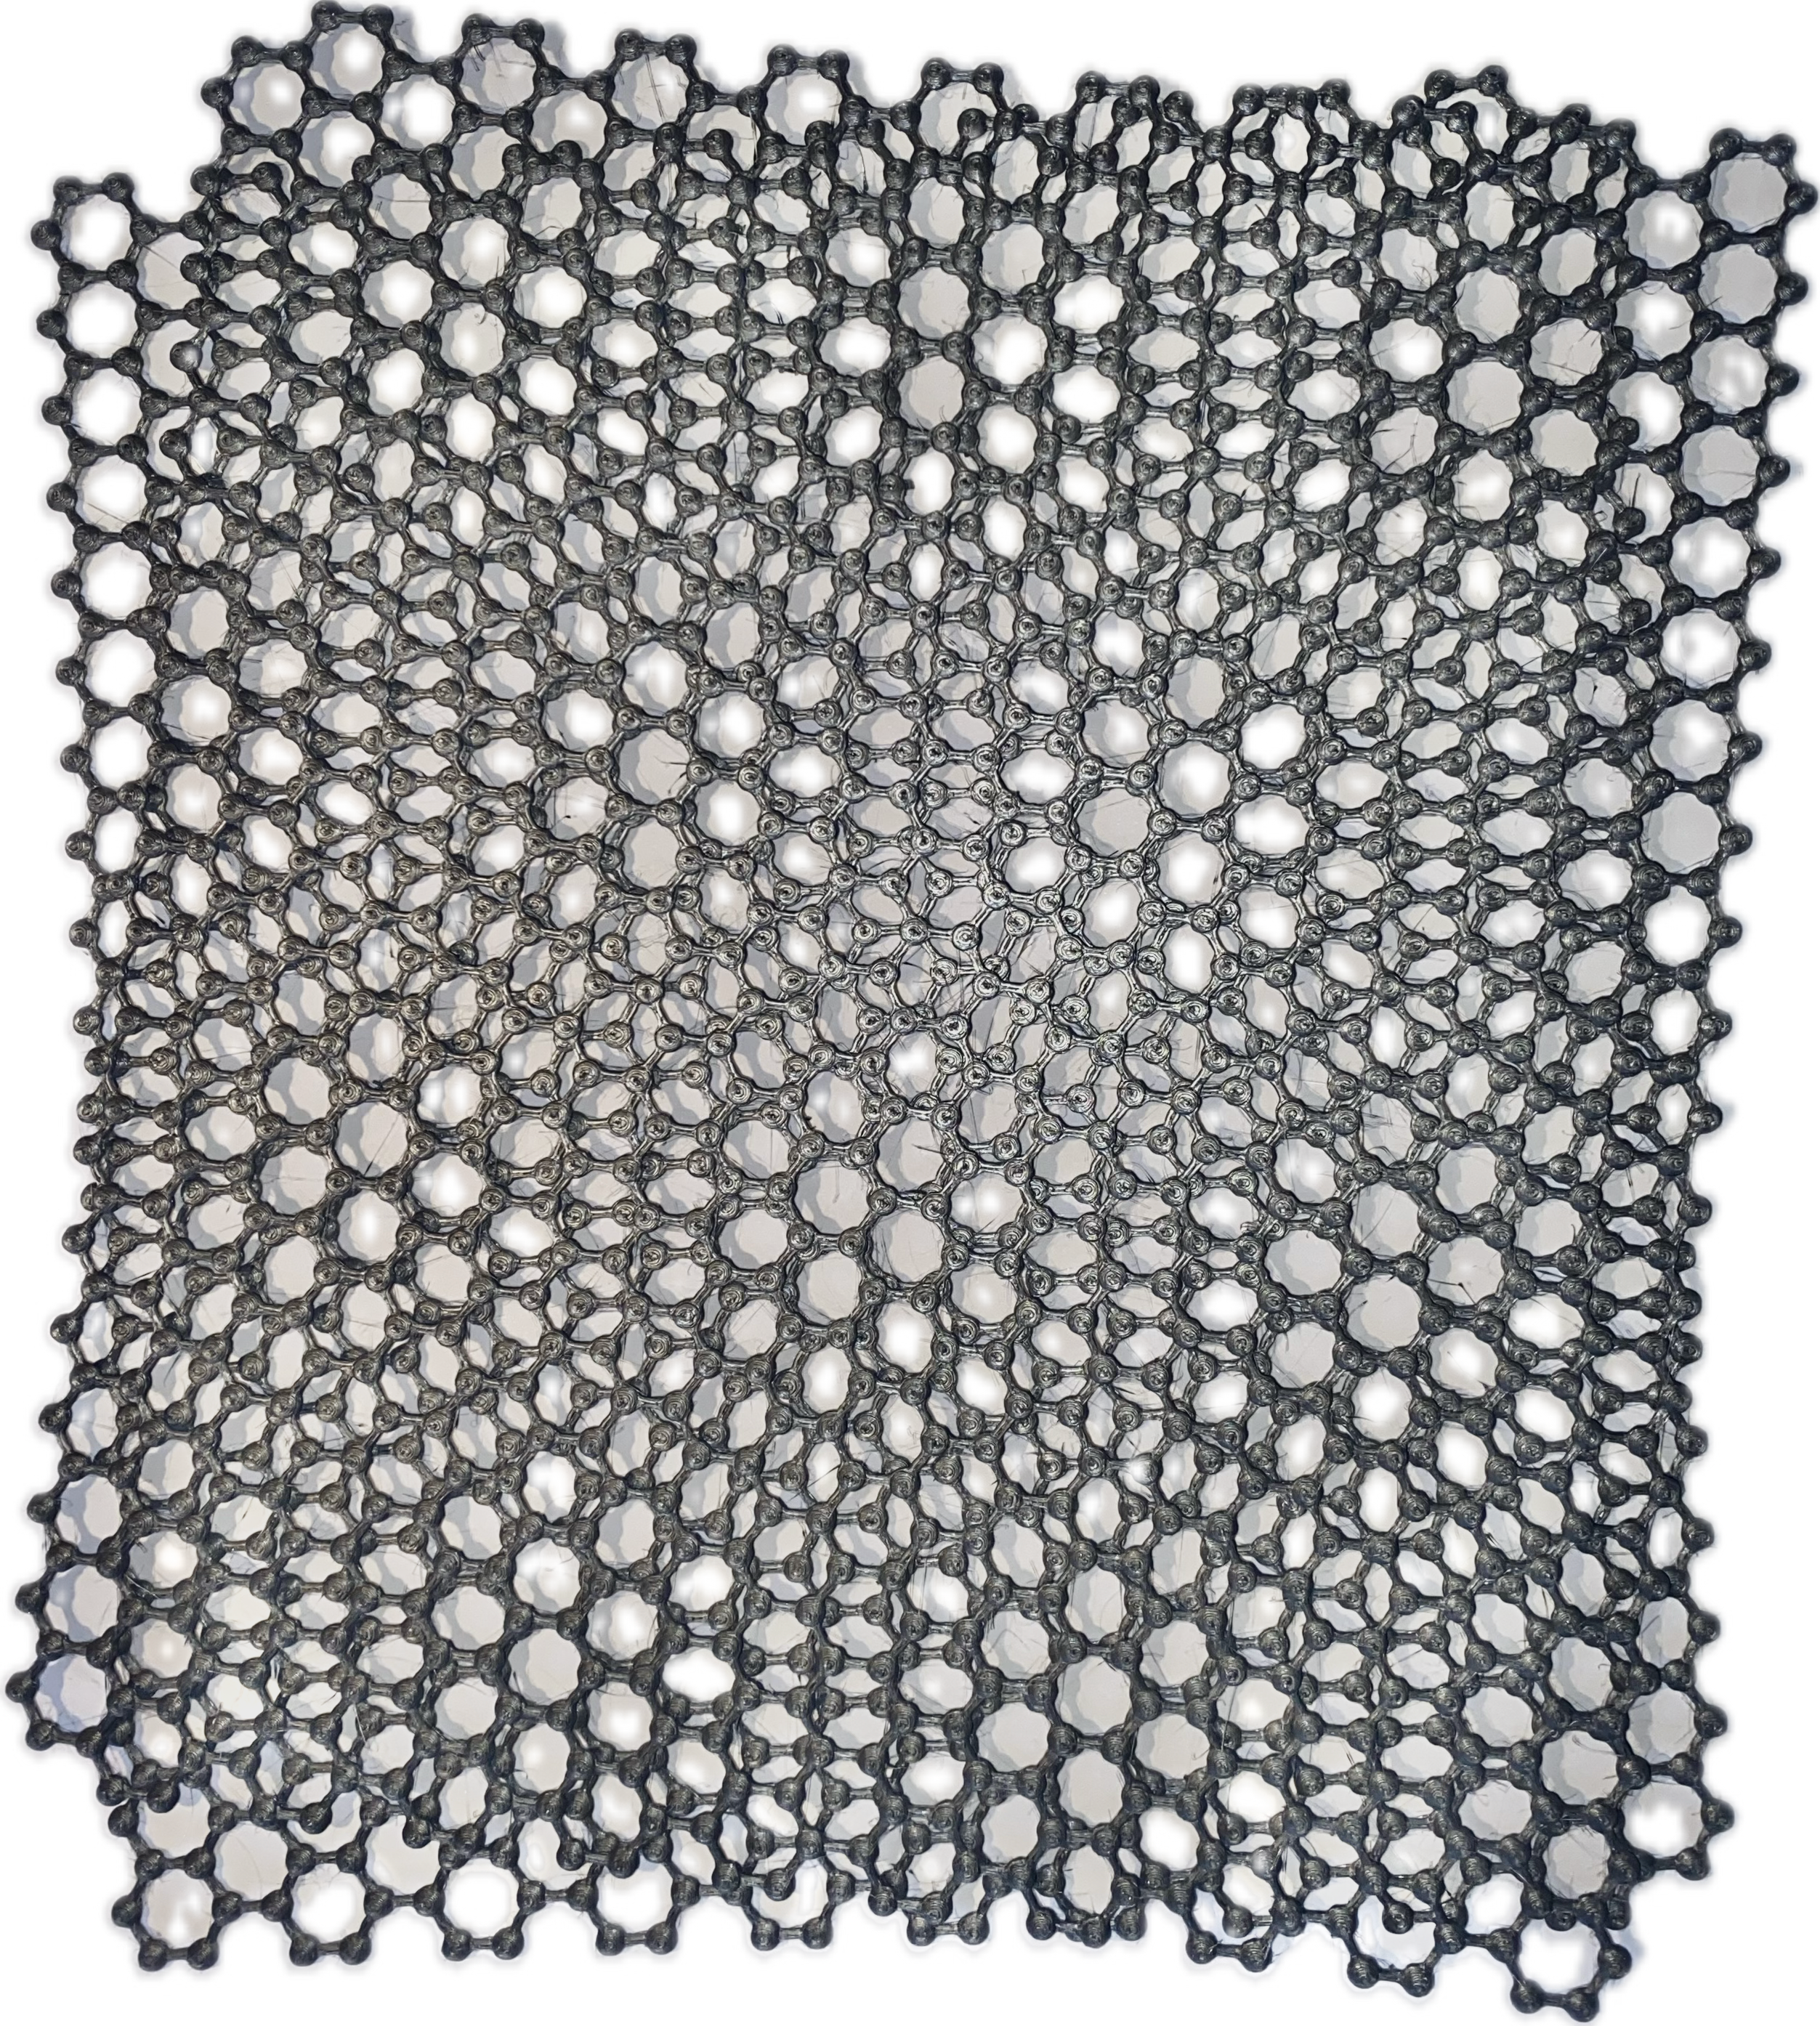
\includegraphics[width=0.75\textwidth]{images/Twisted 3D printed Graphene.png}
	\end{subfigure}%
	\begin{subfigure}[b]{0.5\textwidth}
		\centering
		\caption{\hfill\null}\label{sfig:unconventional SC MATBG}
		\includegraphics[width=1.0\textwidth]{images/cao_unvoncentional_SC_MATBG.png}
	\end{subfigure}%
	\caption{\textbf{(\subref{sfig:3D printed twisted Graphene})} Twisted Bilayer Graphene \textbf{(\subref{sfig:unconventional SC MATBG})} Reproduced from \cite{caoUnconventionalSuperconductivityMagicangle2018} with permission from Springer Nature.}
\end{figure}

\subsection*{Organization of this thesis}

\cref{ch:superconductivity} 

\cref{ch:decorated graphene model}

\cref{ch:results}

\cref{ch:conclusion}

\end{document}